\section{Evaluating Depth-Based Tie-Breaking}
\label{sec:depth-based-evaluation}

% this text is mostly repeated below, so deleted this and promoted the subsection below up 1 level.
%% We evaluated our depth-based diversifying tie-breaking strategies against standard
%% tie-breaking strategies.
%% In addition to the 35 IPC benchmark domains with 1104 instances used in
%% the previous set of experiments, we used 28 Zerocost domains with 620
%% instances.  

%\subsection{Evaluating Depth-Based Tie-Breaking with $h$ tie-breaking}

We compared the performance of standard tie-breaking methods to depth-based tie-breaking methods. These all use $h$
as the second-level sorting criterion and either \fifo, \lifo or \ro (random order) default tie-breaking criterion.
The only difference is the presence of the third, depth-diversification criterion.

Experiments are conducted on {1104 standard IPC benchmark
instances} from 35 domains  and {620 Zerocost instances} from 28 domains (see \refsec{sec:eval-common-strategies} and \refsec{sec:zerocost-domains} for full lists of these domains). 
The basic experimental settings are the same as the previous ones:
Each experiment uses the Fast Downward planner using \astar search and either the \lmcut heuristic or \mands heuristic.
Each experiment is run for 5 minutes excluding SAS translation time, with 4GB memory constraints.

We first show the summary results of these experiments (\reftbl{tbl:depth-summary}).
Overall, depth-based tie-breaking tends to show larger coverages than the
standard tie-breaking strategies.
Interestingly, when the depth diversity criterion $\depth$ is used, 
the performance relationship between \lifo and \fifo seems to flip:
\fifo tends to perform better than \lifo in Zerocost domains for both
\lmcut and \mands heuristics (299 vs 279 for \lmcut, 317 vs 303 for \mands).
Also, \ro (random order) outperforms both \fifo and \lifo.
In the following, we describe and discuss each experiment.
Detailed data tables are in the Appendix (\refsec{sec:appendix}).

\begin{table}[htb]
 {
 \centering
 \setlength{\tabcolsep}{3pt}
 \begin{center}
\begin{tabular}{|l|cc|cc|}
Sorting Criteria & Zerocost(620) & Zerocost(620) & IPC(1104) & IPC(1104)\\
 & \lmcut & \mands & \lmcut & \mands\\
Standard &  &  &  & \\
\([f,h,\fifo]\) & 256 & 280 & 558 & 491\\
\([f,h,\lifo]\) & 279 & 301 & 565 & \textbf{496}\\
\([f,h,\ro]\) & 261.9 \(\pm\) 1.4 & 287.7 \(\pm\) 3.2 & 558.9 \(\pm\) 2.1 & 489.4 \(\pm\) 1.0\\
 &  &  &  & \\
Depth-based &  &  &  & \\
\([f,h,\depth,\fifo]\) & 284 & 302 & 571 & 487\\
\([f,h,\depth,\lifo]\) & 264 & 288 & \textbf{575} & 487\\
\([f,h,\depth,\ro]\) & \textbf{288.1 \(\pm\) 1.6} & \textbf{308.1 \(\pm\) 2.1} & 571.4 \(\pm\) 1.7 & 485.6 \(\pm\) 1.5\\
\end{tabular}
\end{center}

 \caption{
 Main summary results: Coverage comparison (number of instances solved in 5min, 4GB, \lmcut/\mands
 heuristics) between standard tie-breaking and depth-based tie-breaking
 ($\depth$). When \lmcut is used, $\depth$ outperforms standard strategies both in IPC
 instances (1104 problems total) and Zerocost instances (620 problems
 total). When \mands is used, $\depth$ outperforms standard strategies
 in Zerocost instances. \textbf{Bold} shows the best configuration.}
 \label{tbl:depth-summary}
 }
\end{table}

\reftbl{tbl:lmcut-zerocost-full} and \reftbl{tbl:mands-zerocost-full} show the number of Zerocost
instances (out of 620) solved by \lmcut and \mands heuristics. In these
Zerocost domains, our proposed method outperforms the traditional tie-breaking methods in both heuristics.
Significant improvements were observed in 10 domains when using \lmcut, and 7 domains when using \mands.

%% Removed in order to reduce the paper length
% In detail,
% \begin{itemize}
%  \item \textbf{10 Domains improved by depth on Zerocost, using \lmcut,} are \pddl{elevators-up} (\ro), \pddl{freecell-move} (\fifo,\ro),
%        \pddl{miconic-up} (all), \pddl{mprime-succumb} (\fifo,\ro), \pddl{pipesnt-pushstart} (\ro), \pddl{pipesworld-pushend} (\ro),
%        \pddl{scanalyzer-analyze} (\lifo), \pddl{storage-lift} (\fifo), \pddl{tpp-fuel} (\fifo,\ro), \pddl{woodworking-cut} (\fifo,\ro).
%  \item \textbf{7 Domains improved by depth on Zerocost, using \mands,} are \pddl{elevators-up} (\ro), \pddl{freecell-move} (\fifo,\ro),
%        \pddl{mprime-succumb} (\fifo,\ro), \pddl{pipesnt-pushstart} (\fifo, \ro), \pddl{pipesworld-pushend} (\ro),
%        \pddl{tpp-fuel} (\fifo,\ro), \pddl{woodworking-cut} (\fifo,\ro).
% \end{itemize}

\reftbl{tbl:lmcut-ipc-full} shows the number standard IPC benchmark instances (out of 1104) solved by the configuration using \lmcut
heuristics. Depth-based tie-breaking ($\depth$) achieves impressive results on \pddl{Openstacks} ($\fifo:2\to 8,\ \lifo:3\to 12,\  \ro:3.9\to 10$) and \pddl{Cybersec} ($\fifo: 11\to 18,\ \ro: 11.7\to 18$) because these
domains contain many instances of 0-cost edges (See
\refig{fig:plateau}).  Most other instances are unaffected by depth-based tie-breaking.  Thus, depth-based
tie-breaking yields better performance in the domains with 0-cost actions, without sacrificing performance in
other domains.

In contrast, \reftbl{tbl:mands-ipc-full} shows that depth-based tie-breaking degrades the performance of
the configuration using \mands when applied to {1104 standard IPC benchmark instances}. This result can be explained as follows.
% %concatenating into single, long paragraph because  otherwise, it seems that almost the entire 1st part of Sec 7 is about the negative result on M&S, giving the wrong impression of the overall results
First,  similar to the case of \lmcut, \pddl{Openstacks} coverage improved for \fifo ($15\to 19$) and \ro ($15.4\to 19$), which is expected according to our analysis of Zerocost domains.
%
Although there was no improvement on \pddl{Cybersec}, this is because 
the coverage of \pddl{Cybersec} is 0 in all \mands configurations, regardless of tie-breaking. Thus, the positive
contribution of depth diversification to the overall score was limited for \mands compared to \lmcut.

Second, with \mands, performance degraded across a wide range of domains due to the low-level overhead of depth-based tie-breaking (i.e., updates to the depth-based bucket data structures).
As shown in \refig{fig:expansion-ratio}, when depth-based tie-breaking was used, the node evaluations rate significantly decreased with the \mands heuristic, 
% across a wide range of domains
while node evaluation rate decreased much less for \lmcut.
This is because  the \mands heuristic is implemented
as an efficient table lookup, and \mands is able to evaluate an order of magnitude larger number of nodes compared to \lmcut.
Thus, even the relatively small overhead incurred by depth bucket updates decreases the node evaluation rate enough to noticeably degrade \mands performance.
\refig{fig:eval-comparison} shows a cumulative coverage plot which shows the number of node evaluations
required to solve IPC instances.
% 
According to \refig{fig:eval-comparison}, the number of evaluations required to solve IPC instances
for  $[f,h,*]$ and $[f,h,\depth,*]$ were almost identical, which is expected because
IPC instances mostly consist of instances with only positive-cost actions which are unaffected by depth-based tie-breaking (as predicted by our analysis in \refsec{sec:depth}).
%We observed differences in \pddl{Openstacks} as expected, because \pddl{Openstacks} contains 0-cost actions.
%(No \pddl{Cybersec} instances were successfully solved using \mands.)
This shows that the coverage degradation on IPC instances when using depth diversification is caused by the low-level overhead. %removed ``purely'' because sometimes it's due to other causes, e.g. pegsol.
% According to \refig{fig:eval-comparison}, the depth diversification does not
% affect the node evaluation in positive-cost domains while it reduced the number of evaluations in Openstacks
% (contains 0-cost operators). Since Cybersec instances were not solved at all, the results are not included. This
% shows that the degradation in the coverage of IPC track observed by depth diversification is purely caused by the
% low-level overhead.
% 

\begin{figure}[htbp]
 \centering
 % \begin{tabular}{cccc}
 %  nodes/sec                  & LMcut      & M\&S       & M\&S slowdown\\
 %  \hline
 %  $[f,h,\lifo]$              & 8.86$\times 10^3$ & 1.37$\times 10^5$ & 100\%\\
 %  $[f,h,\depth,\lifo]$ & 9.37$\times 10^3$ & 1.13$\times 10^5$ & 82\%\\
 %  \hline
 %  $[f,h,\fifo]$              & 9.65$\times 10^3$ & 1.41$\times 10^5$ & 100\%\\
 %  $[f,h,\depth,\fifo]$ & 9.62$\times 10^3$ & 1.24$\times 10^5$ & 87\%\\
 %  \hline
 % \end{tabular}
 % \caption{Comparison of the average node expansion ratio (node/sec) between
 % standard tie-breaking and depth-based tie-breaking on \lmcut and \mands
 % heuristics. Numbers are averaged over the problem instances solved by
 % all 4 configurations. Since the node evaluation of \mands is an order of
 % magnitude faster than \lmcut, the overhead of managing depth-based
 % tie-breaking queue is non-negligible on \mands.}
 % 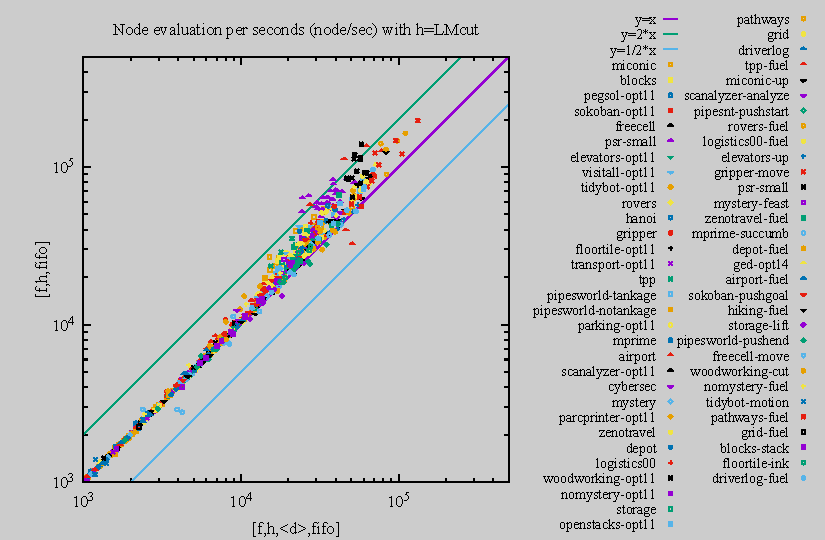
\includegraphics{img/node-sec/lmhiF-lmh_F.pdf}
 % % 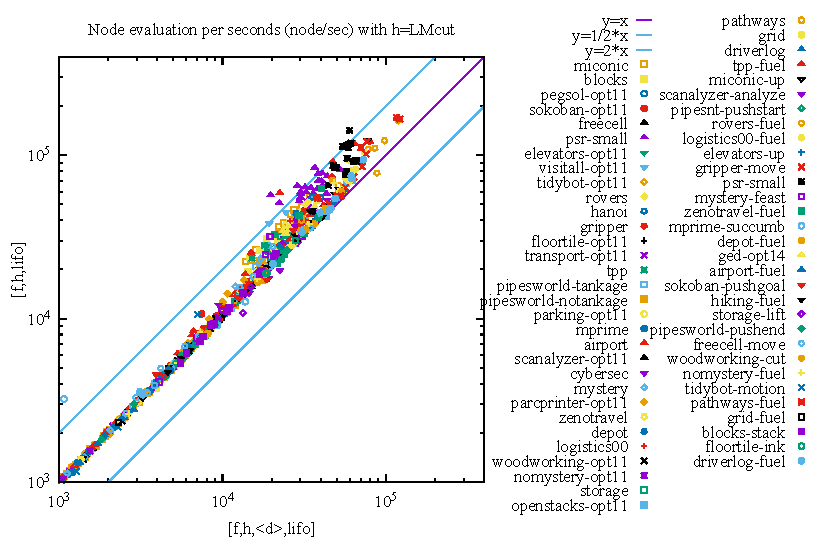
\includegraphics{img/node-sec/lmhiL-lmh_L.pdf}
 % 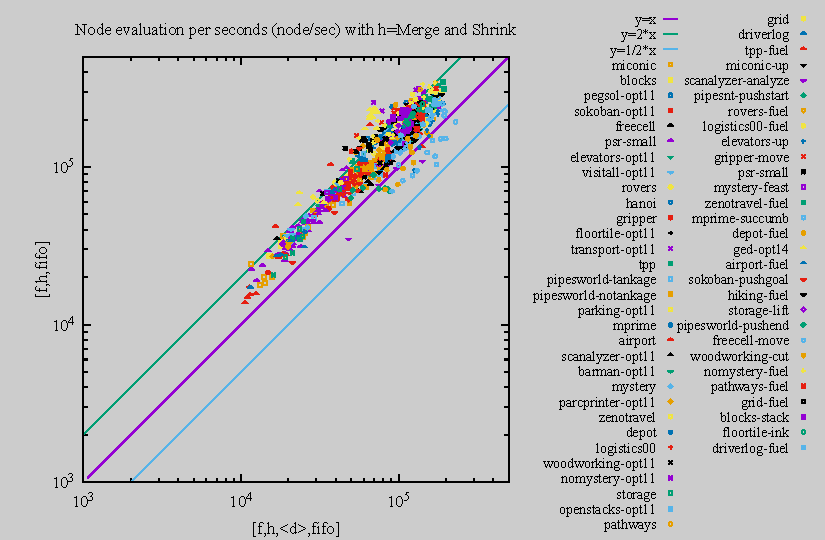
\includegraphics{img/node-sec/mnhiF-mnh_F.pdf}
 % % 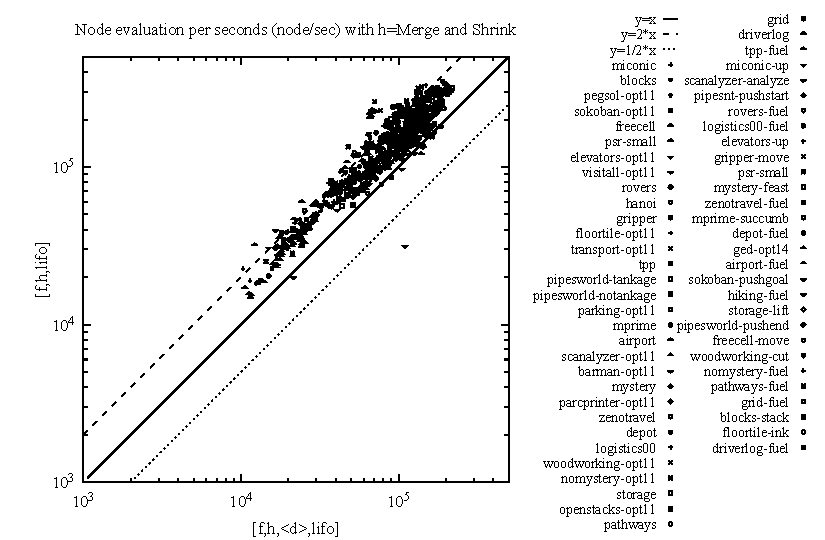
\includegraphics{img/node-sec/mnhiL-mnh_L.pdf}
 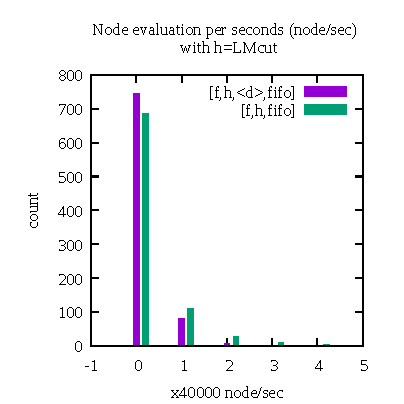
\includegraphics{img/node-sec/lmhiF-lmh_F-hist.pdf}
 % 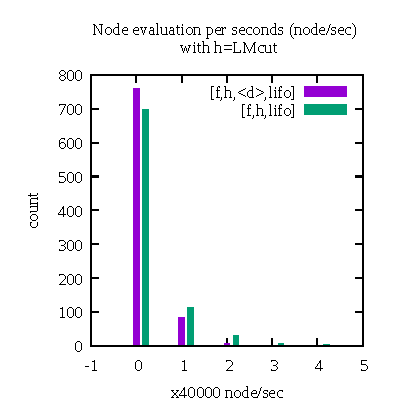
\includegraphics{img/node-sec/lmhiL-lmh_L-hist.pdf}
 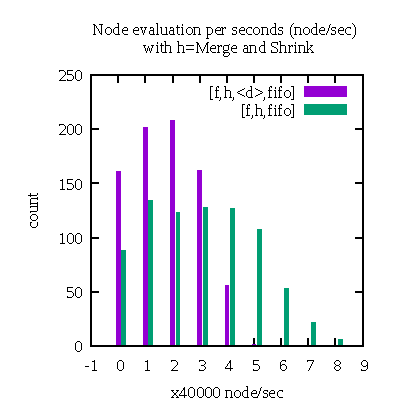
\includegraphics{img/node-sec/mnhiF-mnh_F-hist.pdf}
 % 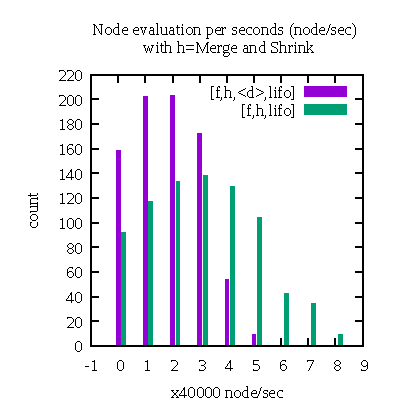
\includegraphics{img/node-sec/mnhiL-mnh_L-hist.pdf}
 % 
 \caption{Histogram comparing the node evaluation ratio (node/sec) between standard tie-breaking ($[f,h,\fifo]$) and
 depth-based tie-breaking ($[f,h,\depth,\fifo]$) on \lmcut and \mands heuristics.
 This plot includes both IPC and Zerocost instances.
 (See Appendix \refig{fig:expansion-ratio-lifo} for the data on $[f,h,\lifo]$ vs. $[f,h,\depth,\lifo]$.)
 On \mands, compared to \lmcut, node evaluation rate more often becomes
 slower when depth is enabled. This is because the node evaluation of \mands is an order of
 magnitude faster than \lmcut, and the overhead of managing depth-based tie-breaking queue becomes significant.
 }
 % 
 \label{fig:expansion-ratio}
\end{figure}


\begin{figure}[htbp]
 \centering
 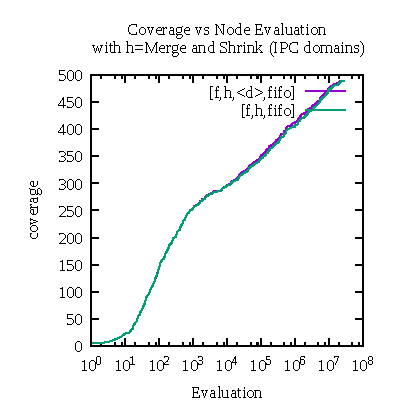
\includegraphics{img/node-sec/mnhiF-mnh_F-benchmark-cumulative.pdf}
 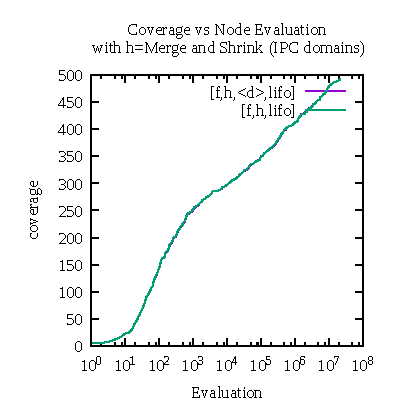
\includegraphics{img/node-sec/mnhiL-mnh_L-benchmark-cumulative.pdf}
 % 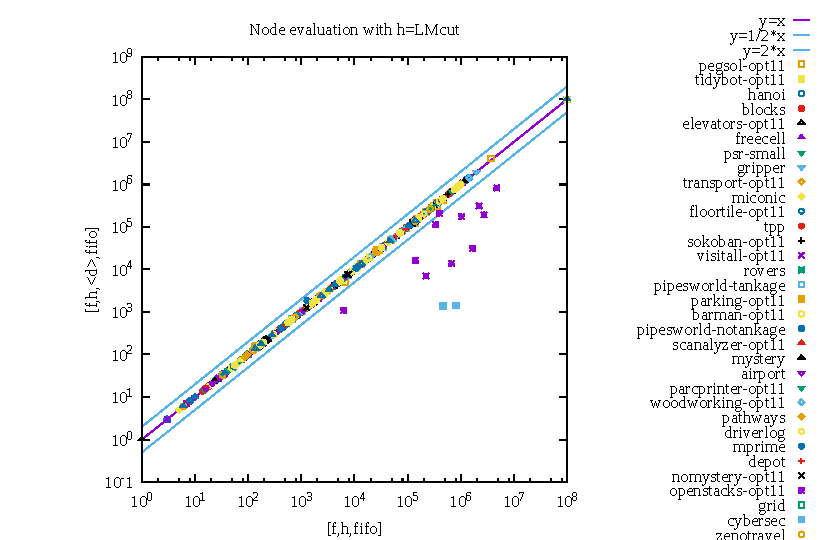
\includegraphics{img/node-sec/lmhiF-lmh_F-eval.pdf}
 % 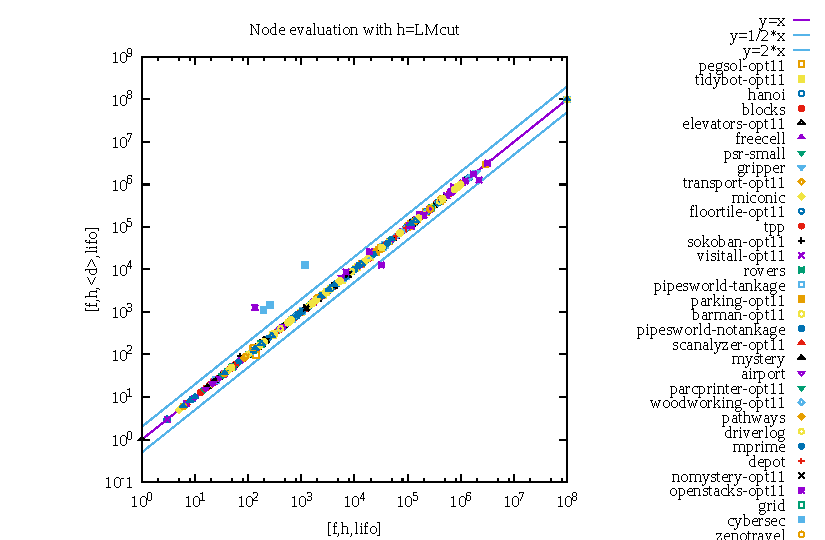
\includegraphics{img/node-sec/lmhiL-lmh_L-eval.pdf}
 % 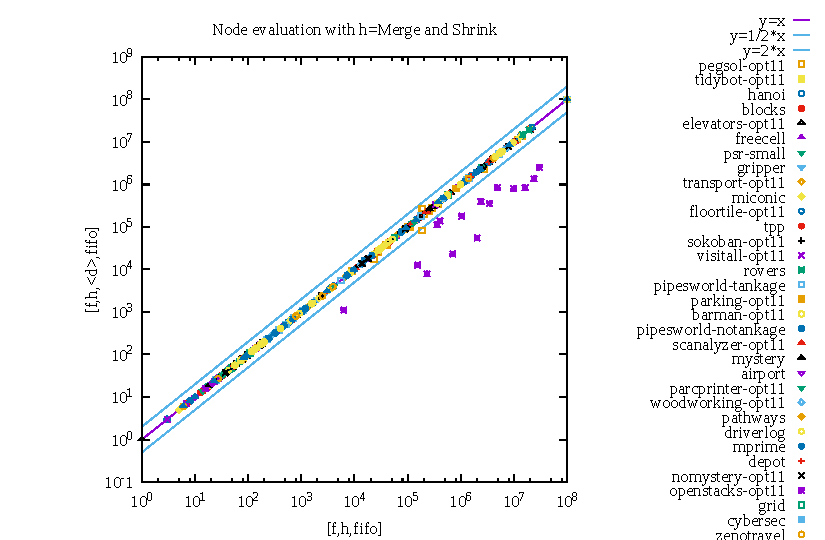
\includegraphics{img/node-sec/mnhiF-mnh_F-eval.pdf}
 % 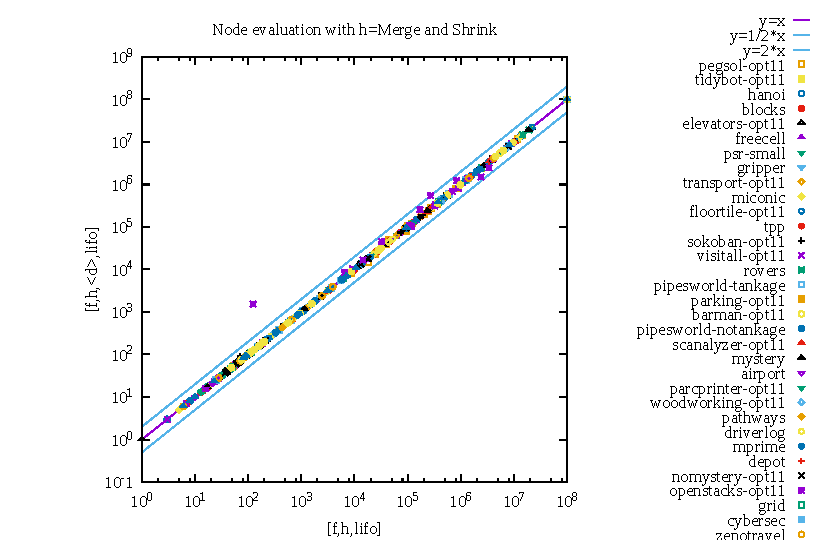
\includegraphics{img/node-sec/mnhiL-mnh_L-eval.pdf}
 % 
 \caption{
 Cumulative coverage ($y$-axis) vs the number of evaluated nodes ($x$-axis),
 on IPC instances solved by both $[f,h,*]$ and $[f,h,\depth,*]$ where $h=\mands$.
 Left: \fifo, Right: \lifo.
 % See \refig{fig:eval-comparison-lifo} for the similar comparison using $\lifo$ default tiebreaking (Appendix).
 % \pddl{Cybersec}(\lmcut only) and \pddl{Openstacks} shows that the evaluation is reduced by depth, \pddl{pegsol-opt11} is slightly affected, but the rest of the domains are while the. For \pddl{Cybersec}, only 2 instances are shown because they are th only instances solved by $[f,h,\fifo]$.
 % There are also slight effect on \pddl{pegsol-opt11} because it also contains zero-cost actions. However, the two 0-cost actions (\pddl{jump-continue-move, end-move}) are the necessary ``finalization'' actions that should always be executed after the unit-cost action (\pddl{jump-start-move}).
 % Due to this domain-specific characteristics, the effect of depth diversification on 0-cost actions are limited on \pddl{pegsol-opt11}.
 }
 % 
 \label{fig:eval-comparison}
\end{figure}

% In contrast, Zerocost domains did not cause such problems to \mands.
% \refig{fig:eval-comparison-zero} shows that the evaluation is significantly decreased on Zerocost domains.
% This shows that the search efficiency offered by depth based diversification becomes much more important, and the low-level overhead became negligible.
% 
% \begin{figure}[htbp]
%  \centering
%  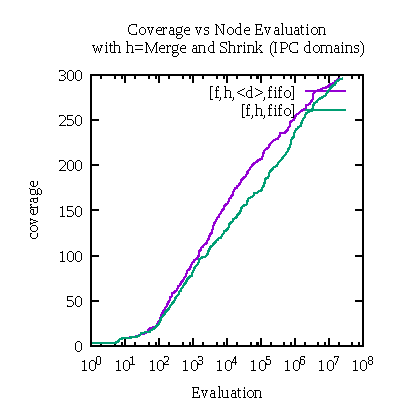
\includegraphics{img/node-sec/mnhiF-mnh_F-zerocost-cumulative.pdf}
%  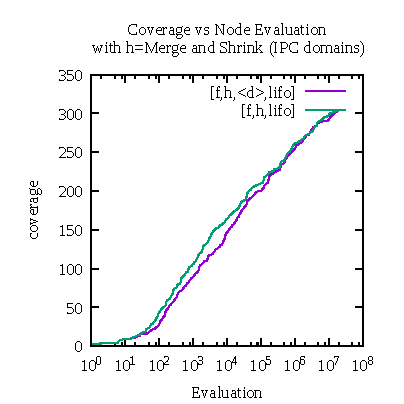
\includegraphics{img/node-sec/mnhiL-mnh_L-zerocost-cumulative.pdf}
%  % 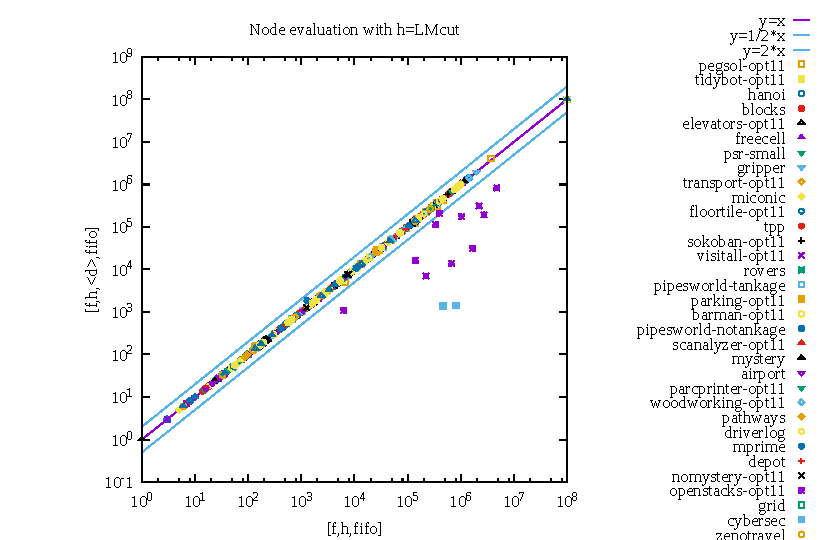
\includegraphics{img/node-sec/lmhiF-lmh_F-eval.pdf}
%  % 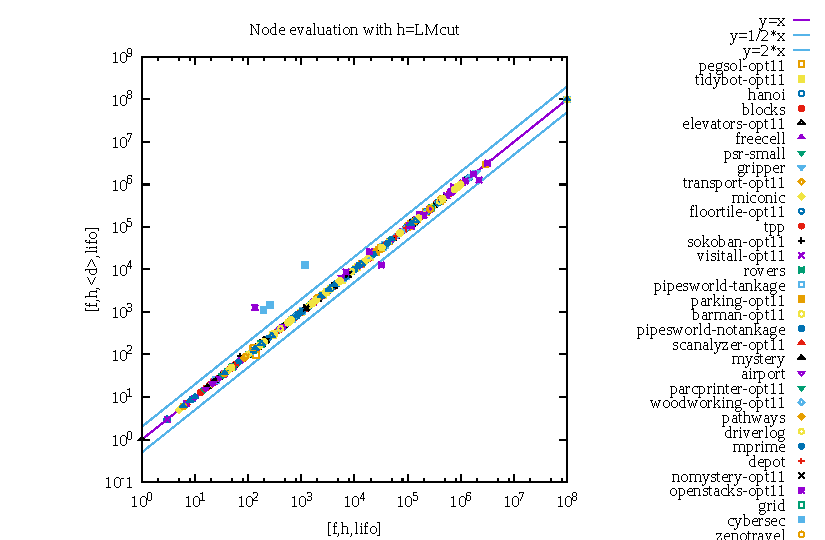
\includegraphics{img/node-sec/lmhiL-lmh_L-eval.pdf}
%  % 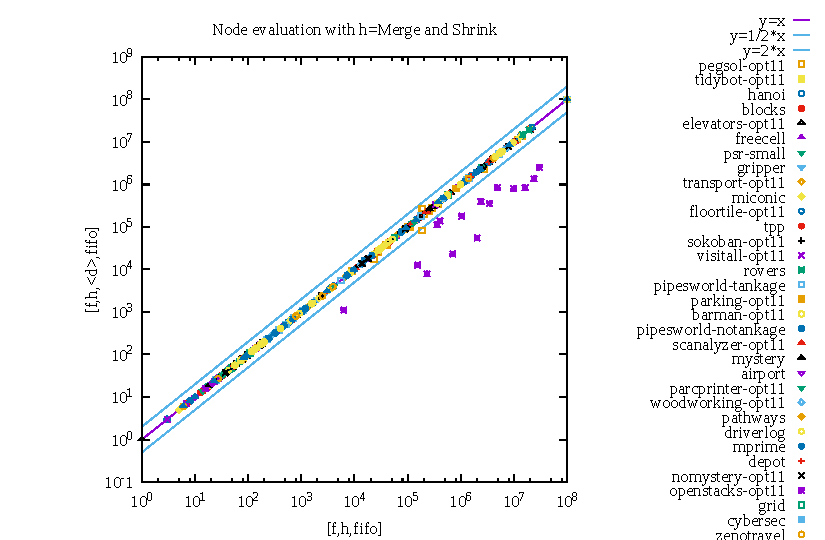
\includegraphics{img/node-sec/mnhiF-mnh_F-eval.pdf}
%  % 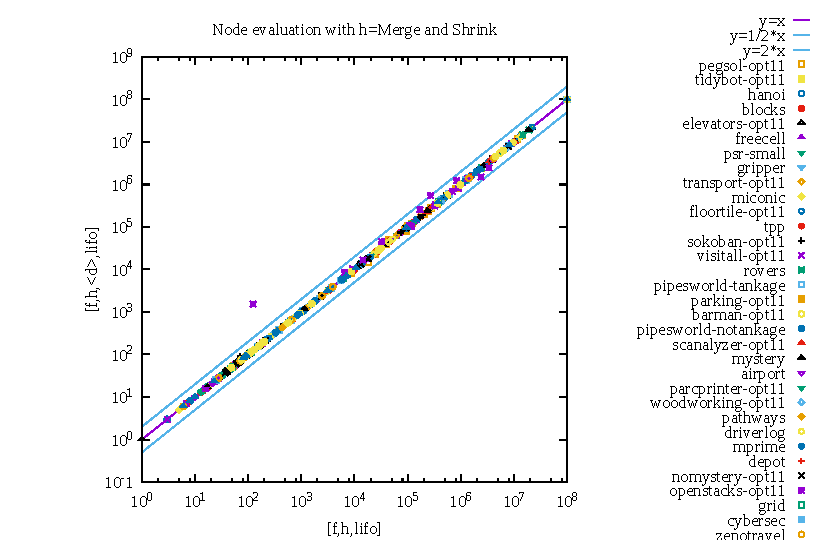
\includegraphics{img/node-sec/mnhiL-mnh_L-eval.pdf}
%  % 
%  \caption{
%  Cumulative coverage ($y$-axis) vs the number of evaluated nodes ($x$-axis),
%  on Zerocost instances solved by both $[f,h,*]$ and $[f,h,\depth,*]$ where $h=\mands$.
%  % See \refig{fig:eval-comparison-lifo} for the similar comparison using $\lifo$ default tiebreaking (Appendix).
%  % \pddl{Cybersec}(\lmcut only) and \pddl{Openstacks} shows that the evaluation is reduced by depth, \pddl{pegsol-opt11} is slightly affected, but the rest of the domains are while the. For \pddl{Cybersec}, only 2 instances are shown because they are th only instances solved by $[f,h,\fifo]$.
%  % There are also slight effect on \pddl{pegsol-opt11} because it also contains zero-cost actions. However, the two 0-cost actions (\pddl{jump-continue-move, end-move}) are the necessary ``finalization'' actions that should always be executed after the unit-cost action (\pddl{jump-start-move}).
%  % Due to this domain-specific characteristics, the effect of depth diversification on 0-cost actions are limited on \pddl{pegsol-opt11}.
%  }
%  % 
%  \label{fig:eval-comparison-zero}
% \end{figure}

Finally, the per-domain results for Zerocost domains (\reftbls{tbl:lmcut-zerocost-full}{tbl:mands-zerocost-full}\todo*{reftables}) show that 
$\depth$ can cause both improvement and degradation (despite the total coverage improvement).
This is natural considering that depth-diversification is designed to be a conservative, domain-independent strategy which is designed to avoid worst-case pathological behaviors.
 Overall,  $\depth$ tends to perform well, but the best-performing strategy on particular domain varies
   --- for example,
 \fifo is the best in \pddl{airport-fuel} with \lmcut, while
 \lifo is the best in \pddl{freecell-move} with \lmcut.
 % However, $\depth$ is the best practice for a domain-independent planner which should avoid pathological behavior in the general cases. % claim too strong
 An adaptive tie-breaking which selects the tie-breaking strategy for a given domain is discussed in \refsec{sec:dynamic-configuration}.

% , which is less interesting when tackling an intractable combinatorial problems.

% \reftbl{tbl:mands-evaluations} shows that if we instead compare the
% number of evaluations on problems solved by both, depth-based
% tie-breaking significantly outperforms the standard tie-breaking
% strategies. Moreover, in the next \textbf{Zerocost} domain experiments,
% depth-based tie-breaking ourperforms the standard tie-breaking
% overall. Besides, the coverages by \mands is less than that of \lmcut.

% \begin{figure}[htb]
%  \centering
%  \caption{
%  Comparison of the total number of nodes generated
%  by \mands heuristics until
%  the goal is found, with vs without depth-based tie-breaking.
%  } \label{tbl:mands-evaluations}
% \end{figure}

\subsection{Search Behavior Within a Plateau}

To understand the behavior of depth-based policies, we plotted 
histograms of the depths of search nodes evaluated by several tie-breaking
strategies in the final plateau $\plateau{f^*,0}$ until the solution is
found.  We plotted a depth-based strategy
$[f,h,\depth,\fifo]$, as well as the standard strategies $[f,h,\fifo]$,
$[f,h,\lifo]$ and a single run of randomized strategy $[f,h,\ro]$.

In order to obtain the data for the strategies which do not use depth-based tie-breaking ($[f,h,\fifo]$, $[f,h,\lifo]$, $[f,h,\ro]$), we added some instrumentation to these strategies so that, the depth of each of the expanded nodes is computed, although they do not affect the search behavior.
Note that this instrumentation, which adds some runtime overhead, was \emph{not}
used in the performance comparison experiments above, and were only used for this experiment, which analyzes search behavior.


\refig{fig:depth-histogram} (as well as \refigs{fig:depth-histogram2}{fig:depth-histogram3} in the Appendix) show the results on exemplary instances from 
various Zerocost domains.  We do not show some domains where we did not observe any depths greater than 3, in which case both
the depth metric and  $\lifo/\fifo/\ro$ have a negligible impact on search performance.
We observed very similar results across a wide range of domains as shown in the figures.
This indicates that the depth metric accurately describes the behavior of each tie-breaking criterion.

For example, consider the first figure, which plots depths searched on \pddl{depot-fuel}, p07.
\todo*{...Instead of only general trends ... mention specific domains to add some ``color''}
% 
The  $[f,h,\lifo]$ plot shows that the depth-first behavior results in deeper search ($\approx 10^3$), while
only a handful of nodes are expanded at intermediate depths (usually once). Thus,  \lifo's depth-first
behavior is prone to  missing the key branch at intermediate depths that may lead to solutions earlier.
On the other hand, the breadth-first behavior of $[f,h,\fifo]$ often gets stuck spending an excessive amount of
time searching around the plateau entrance (expanding $\approx 10^3$ nodes at depth 10).

Also, we noticed that the node distribution of the global randomization $[f,h,\ro]$ is very similar to $[f,h,\fifo]$.
This shows that \ro actually behaves very similar to \fifo, which is consistent with the previous performance comparisons in \refsec{sec:eval-common-strategies} and our observation regarding \ro in \refsec{sec:depth}.
Thus, the overall behavior of \ro tends to be similar to \fifo, and naive randomization does not solve the problem of heavy bias for shallower depth nodes.

In contrast, $[f,h,\depth,\fifo]$ is balancing the search at various depths.
The yellow curve representing $[f,h,\depth,\fifo]$ tends to be almost flat at shallow depths while gradually decreasing the number of nodes at larger depths.
Moreover, its node distribution almost accurately follows $D-d$, a theoretical model from \refsec{sec:theoretical-characteristics} which applies the simplified
assumption that the plateau is a forest with a fixed branching factor.
$D$ denotes the largest depth of the unexpanded nodes in the final plateau, which is
1 larger than the largest depth of the expanded nodes.

The discrepancy of the $[f,h,\depth,\fifo]$ curve from the theoretical prediction $D-d$ can be caused by the 
following factors: First, the outdegree of each node in the graph may not be
uniform across the search space. Second, some depth buckets could be
exhausted, as depicted in the  $[f,h,\fifo]$ line which
shows that all nodes in the shallower depths are expanded while the line is still below $D-d$.
Since $[f,h,\fifo]$ exhaustively expands the nodes in shallower depth,
the number of expansion by $[f,h,\fifo]$ in the shallower depths constitutes an upper bound, which may be below $D-d$.

Next, \refig{fig:depth-histogram4} shows the same results on the standard IPC
\pddl{Openstacks} and \pddl{Cybersec} domains.
The \pddl{Openstacks} results were similar to those of the Zerocost domains.
In \pddl{Cybersec},
% while the depth has improved the overall performance,
we found that the performance improvement was not due to the number of nodes in $\plateau{f^*,0}$,  because all tie-breaking strategies have generated only a small number of such nodes before the solution was found.
Instead, we observed a large difference in the depth distributions in non-final plateaus $\plateau{f^*,h}, h\not=0$ caused by the difference of tie-breaking.
Note that depth diversification is always applied regardless of $f$ or $h$ values.
This suggests that most children of the nodes in $\plateau{f^*,h}$ have $f$ value larger than $f^*$ or stays in $\plateau{f^*,h}$, and the planner is struggling to find nodes with better $h$.
Due to the unbiased search, the depth-based strategy has a better chance of improving $h$ values, finding a node in $\plateau{f^*,0}$ more quickly.
This shows that considering depth can also help the search in non-final plateaus to find the nodes in the next plateau.
Similar phenomena were observed in several other instances and domains, e.g., \pddl{depot-fuel}, \pddl{driverlog-fuel}, \pddl{zenotravel-fuel}, \pddl{floortile-ink}, \pddl{mprime-succumb}, \pddl{storage-lift} (\refig{fig:depth-histogram5} in Appendix).
\todo*{might as well say which domains...}

Note that the small number of nodes in $\plateau{f^*,0}$ in this experiment does not contradict the results in \refig{fig:plateau},  which shows that  the number of such nodes is quite large.
This is because, while in \refig{fig:plateau} the search continues until expanding all nodes in the final plateau, in this experiment the search stops when the first solution is found --  \refig{fig:plateau} was intended to show the size of the entire final plateau, while \refigs{fig:depth-histogram}{fig:depth-histogram4} were meant to show the actual search behavior. If we continue the search until exhausting the final plateau, all tie-breaking strategies will expand the same set of nodes (in different orders), so we would obtain plots similar to \refig{fig:plateau} regardless of the tie-breaking strategy.

\begin{figure}[htbp]
% 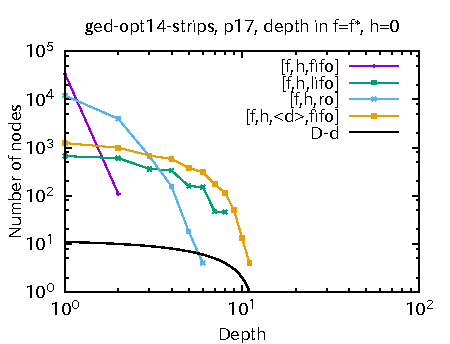
\includegraphics{img/output-lmcut/ged-opt14-strips/p17-0.pdf}
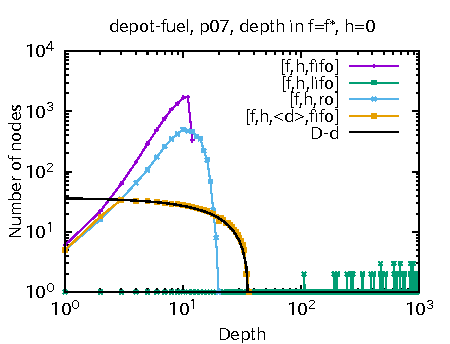
\includegraphics[width=0.49\linewidth]{img/output-lmcut/depot-fuel/p07-0.pdf}
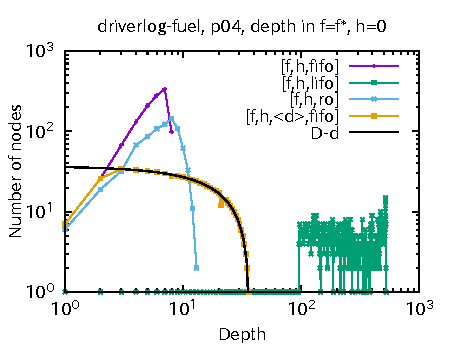
\includegraphics[width=0.49\linewidth]{img/output-lmcut/driverlog-fuel/p04-0.pdf}
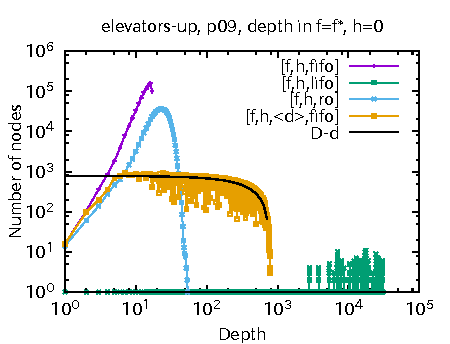
\includegraphics[width=0.49\linewidth]{img/output-lmcut/elevators-up/p09-0.pdf}
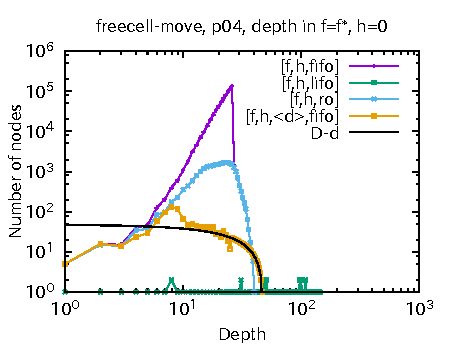
\includegraphics[width=0.49\linewidth]{img/output-lmcut/freecell-move/p04-0.pdf}
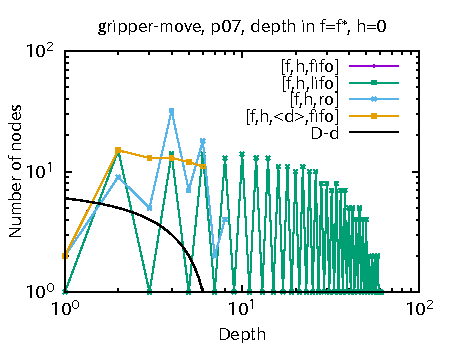
\includegraphics[width=0.49\linewidth]{img/output-lmcut/gripper-move/p07-0.pdf}
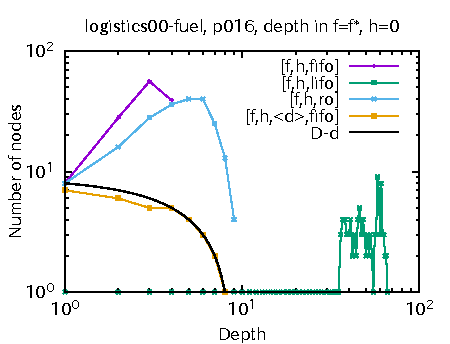
\includegraphics[width=0.49\linewidth]{img/output-lmcut/logistics00-fuel/p016-0.pdf}
 \caption{Number of nodes ($y$-axis) expanded per depth ($x$-axis) in
 the final plateau with different tie-breaking strategies. Both axes are in logarithmic scale.
 }
 \label{fig:depth-histogram}
\end{figure}

\begin{figure}[htbp]
\begin{center}
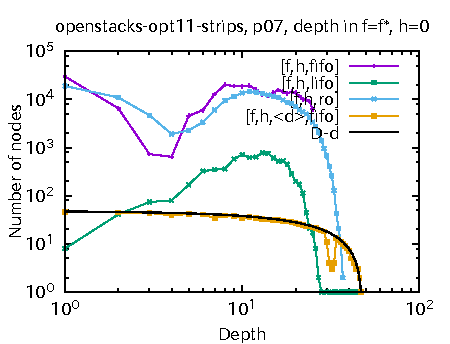
\includegraphics{img/output-lmcut/openstacks-opt11-strips/p07-0.pdf}
\end{center}

% 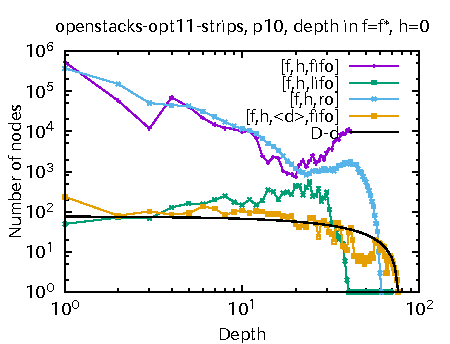
\includegraphics{img/output-lmcut/openstacks-opt11-strips/p10-0.pdf}
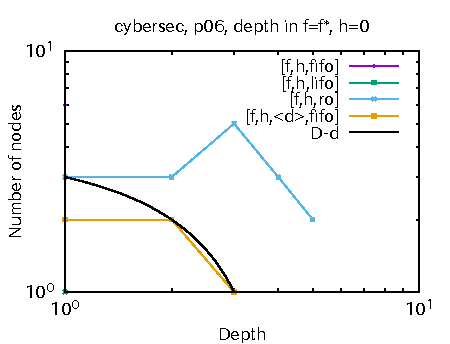
\includegraphics[width=0.49\linewidth]{img/output-lmcut/cybersec/p06-0.pdf}
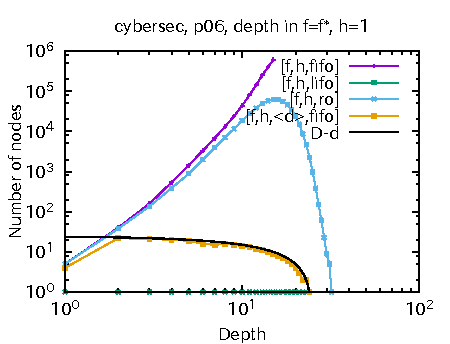
\includegraphics[width=0.49\linewidth]{img/output-lmcut/cybersec/p06-1.pdf}
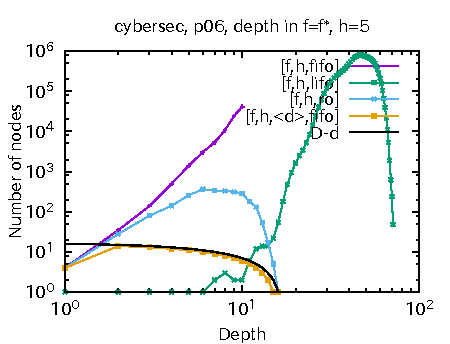
\includegraphics[width=0.49\linewidth]{img/output-lmcut/cybersec/p06-5.pdf}
% 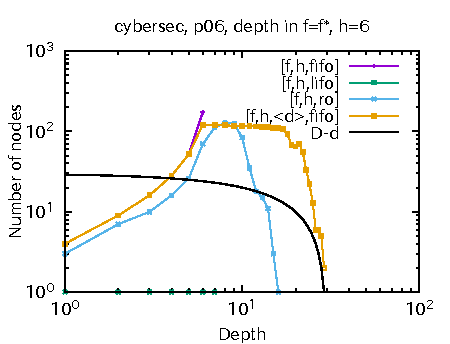
\includegraphics{img/output-lmcut/cybersec/p06-6.pdf}
% 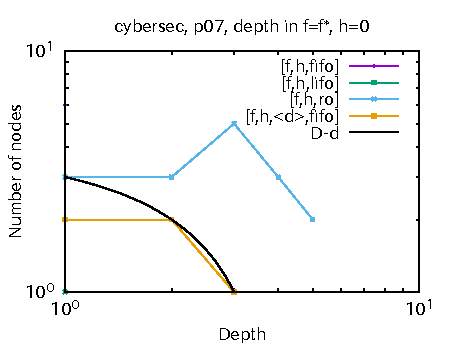
\includegraphics{img/output-lmcut/cybersec/p07-0.pdf}
% 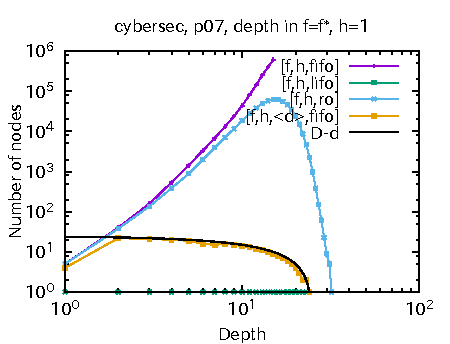
\includegraphics{img/output-lmcut/cybersec/p07-1.pdf}
% 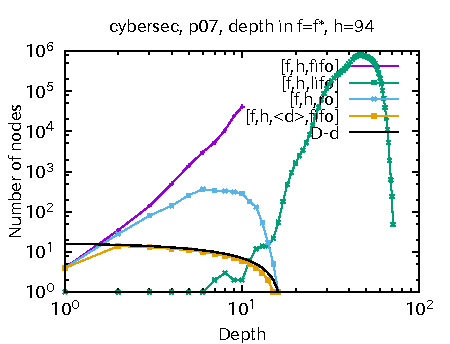
\includegraphics{img/output-lmcut/cybersec/p07-94.pdf}
% 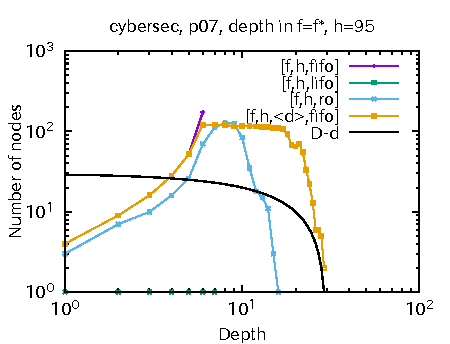
\includegraphics{img/output-lmcut/cybersec/p07-95.pdf}
 \caption{Depth distribution of \pddl{Openstacks} and \pddl{Cybersec} instances in the final ($\plateau{f^*,0}$) and non-final plateaus ($\plateau{f^*,h}, h\not=0$). In \pddl{Cybersec} p06, although the number of nodes generated in $\plateau{f^*,0}$ is small, \fifo and \ro behaved poorly on $\plateau{f^*,1}$, and also \lifo behaved poorly on $\plateau{f^*,5}$.
 % The same behavior was observed in p07.
 }
 \label{fig:depth-histogram4}
\end{figure}




\subsection{The Effect of Domain Mangling}

\label{sec:mangling}

%%%%%%%%%%%%%%%%%%%%%%%%%%%%%%%%%%%%%%%%%%%%%%%%%%%%5

We tested the robustness of the standard $[f,h,\lifo]$ and $[f,h,\fifo]$ strategies, as well as $[f,h,\depth,\ro]$,
with respect to 
biases introduced by domain configuration (action naming) in the PDDL domain definition.
We created 3 different sets of domains in which the
original names of action schema are mangled into random strings. 
%We only reordered the actions because in the FD codebase, the order of propositions has no effect on tiebreaking. --- let's avoid talking about anything other than action names, in case there are other configuration factors.
%  XXXTODO CHECK whether above sentence correctly summarizes the sentence below.
%% In contrast, we continued to use the variable ordering in the original domains
%% because the effect of variable ordering is irrelevant to the tiebreaking
%% criteria.
% %We avoided the effect of action orderings by using the randomized third tiebreaking.
%Each set of action-renamed domains contains all of the benchmark and zerocost domains.   %XX - can be inferred from table
We ran each of the 3 strategies on each
set of mangled domains, three times each with different random seeds,
resulting in 9 runs per strategy.
% (recall that robustness wrto random seed was shown in \refsec{sec:depth-based-evaluation}.)

\begin{table}[htbp]
 \centering \relsize{-1}
 \begin{tabular}{|c|c|c||c|}
\hline         
 Domain & $[h,\fifo]$ & $[h,\lifo]$   & \spc{$[h,\rd,\ro]$ \\($n$: number of runs)}    \\
\hline         
 Mangled IPC 1 (1104) &  556 &  564 &  571.7\spm{}0.9 ($n=3$)\\\hline
 Mangled IPC 2 (1104) &  557 &  568 &  571.3\spm{}0.9 ($n=3$)\\\hline
 Mangled IPC 3 (1104) &  557 &  568 &  573.0\spm{}1.6 ($n=3$)\\\hline
 Original IPC (1104) &  558 &  565 &  570.6\spm{}1.5 ($n=10$)\\\hline
 Mangled Zerocost 1 (620) &  256 &  277 &  288.7\spm{}3.7 ($n=3$)\\\hline
 Mangled Zerocost 2 (620) &  256 &  277 &  285.0\spm{}0.8 ($n=3$)\\\hline
 Mangled Zerocost 3 (620) &  256 &  279 &  286.7\spm{}0.9 ($n=3$)\\\hline
 Original Zerocost  (620) &  256 &  279 &  287.2\spm{}2.4 ($n=10$)\\\hline
\end{tabular}

 \caption{Total coverages of $[f,h,\fifo]$, $[f,h,\lifo]$
 and $[f,h,\depth,\ro]$ (with three seeds). Each row represents the original set of
 domains or its three action-mangled variants. The effect
 of action ordering is small enough for $[f,h,\depth,\ro]$ to
 constantly perform better than the traditional tiebreaking methods.
Note: We used the randomized version of $\depth$ in this experiment.
}
 \label{actionordering-robustness}
\end{table}

The results are shown in \reftbl{actionordering-robustness}.
We statistically analyzed the results for $[f,h,\depth,\ro]$ 
to see if any of the 4 sets of domains
significantly outperformed the others.
%In order to test the significance of mean value,
Fligner-Killeen's non-parametric test could not reject the homogeneity of variances
($p=0.75$ for IPC, $p=0.26$ for Zerocost), so
% Since the variances were not significantly different,
we then applied the non-parametric Kruskal-Wallis test,
% to see if there is any difference in the mean values between the original
% population of the sample groups, 
which showed that the mean differences were not significant
($p=0.28$ for IPC, $p=0.44$ for Zerocost),
% We first applied Fligner-Killeen's non-parametric test to see if the sample groups 
% in each set of randomized domains share the same variance, 
% but could not reject the homogeneity of variances ($p=0.74$).
% Since the variances were not significantly different,
% we could then apply the non-parametric Kruskal-Wallis test to see if
% there is any difference in the mean values between the original
% population of the sample groups, which showed that the differences were not significant ($p=0.26$),
i.e., action name mangling did not significantly affect performance.

Thus, in contrast to the results for satisficing search by \cite{vallati2015effective}, 
the effect of action ordering  seems to be relatively weak for cost-optimal search using \astar.
This may be because 
compared to the satisficing, best-first search algorithms evaluated in \cite{vallati2015effective},
the behavior of admissible search is more constrained.
% $[f,h,\lifo]$, $[f,h,\fifo]$, and $[f,h,rd,\ro]$ are
% because of the first-level tiebreaking according to $h$.
%in that all nodes with cost $f$ must be expanded before any nodes with cost larger than $f$.
% this is true for best-first-search in general, by definition.

%%%%%%%%%%%%%%%%%%%%%%%%%%%%%%%%%%%%%%%%%%%%%%%%%%%%%%%%%%%%%%%%

% Recent work showed that the performance of a satisficing planner can be
% significantly affected by the order in which actions appear in a PDDL
% file \cite{vallati2015effective}.
% However, the conference version of this paper \cite{Asai2016} showed that
% the effect of such an accidental bias is not statistically significant in cost-optimal search,
% by comparing the performance on
% several sets of randomly ``mangled'' domains whose action names are replaced with random strings.
% Moreover, the \ro default tie-breaking should be unaffected by such an accidental bias.
% Thus, we believe it is safe to claim that the experimental results in
% this paper are not a product of such accidental biases.
